\documentclass[aspectratio=169]{beamer}
\usepackage[T1]{fontenc}
\usepackage[utf8]{inputenc}
\usepackage[brazil]{babel}
\usepackage{lmodern,booktabs,amsmath,graphicx,tikz}
\usetikzlibrary{arrows.meta,positioning}
\IfFileExists{beamerthemeInf.sty}{\usetheme{Inf}}{\usetheme{Madrid}}
\providecommand{\InfTitlePage}{\begin{frame}[plain]\titlepage\end{frame}}
\title[Pomodoro adaptativo]{Quando vale a pena adaptar um ciclo Pomodoro?}
\subtitle{Aprendizado por reforço em um simulador de estudo e pausa}
\author{}
\date{}
\newcommand{\fonte}[1]{\par\smallskip{\scriptsize\color{black!70}Fonte: #1.\par}}
\newcommand{\notebook}{\texttt{notebooks/02\_sensibilidade.ipynb}}
\begin{document}
\InfTitlePage

\begin{frame}{Roteiro}
\tableofcontents
\end{frame}

\section{Pergunta de pesquisa}
\begin{frame}{Quanto estudar antes da próxima pausa?}
Um bloco mais longo oferece mais minutos de estudo agora. Se a fadiga persistir após a pausa, o próximo bloco pode render menos.
\begin{alertblock}{Pergunta}
Uma política que considera os próximos ciclos consegue mais minutos efetivos por hora e menos relatos de cansaço alto que um bandit contextual e um ciclo curto fixo?
\end{alertblock}
\begin{itemize}
\item \textbf{Hipótese sobre o horizonte.} Antecipar recompensas futuras pode favorecer o Q-learning frente ao bandit.
\item \textbf{Hipótese sobre adaptação.} Usar cansaço e urgência para escolher o ciclo pode superar a repetição de 15 minutos de estudo e 5 de pausa.
\end{itemize}
\end{frame}

\section{Simulador e políticas}
\begin{frame}{O agente decide oito vezes por sessão}
\begin{columns}[T,onlytextwidth]
\column{.57\textwidth}
\begin{block}{O que o agente observa}
O autorrelato varia de 1 a 5. A urgência pode ser \emph{longe}, \emph{semana} ou \emph{véspera} e permanece constante na sessão. A tabela distingue $5\times3=15$ observações.
\end{block}
A fadiga real $F\in[0,1]$ é latente. Dois ciclos com o mesmo relato podem começar com fadigas diferentes.
\column{.39\textwidth}
\begin{block}{Ações disponíveis}
\centering
\begin{tabular}{lrr}
\toprule Ciclo & Estudo & Pausa\\ \midrule
Curto & 15 & 5\\
Padrão & 25 & 5\\
Foco & 50 & 10\\ \bottomrule
\end{tabular}\par\smallskip
Duração em minutos.
\end{block}
\end{columns}
\medskip A sessão começa com $F$ uniforme entre 0 e 0,3 e termina após a oitava pausa.
\end{frame}

\begin{frame}{Como um ciclo altera a próxima decisão}
\centering
\begin{tikzpicture}[node distance=0.48cm,box/.style={draw=blue!55!black,fill=blue!6,rounded corners,align=center,minimum height=12mm,text width=2.55cm},link/.style={-{Stealth},thick}]
\node[box] (a) {Escolha do ciclo};
\node[box,right=of a] (b) {Estudo\\acumula fadiga};
\node[box,right=of b] (c) {Pausa\\reduz fadiga};
\node[box,right=of c] (d) {Novo relato\\de cansaço};
\draw[link] (a)--(b);\draw[link] (b)--(c);\draw[link] (c)--(d);
\draw[link] (d.south) -- ++(0,-.42) -| (a.south);
\end{tikzpicture}
\begin{itemize}
\item No minuto $t$ do bloco ($t=0,1,\ldots$), a fadiga cresce em $f\,m_u(1+t/25)$, até 1. O multiplicador de urgência $m_u$ vale 1, 1,10 ou 1,25.
\item Cada minuto de pausa reduz a fadiga em $r$, até o piso zero.
\item Após a pausa, o simulador soma ruído normal ($\sigma=0{,}35$) a $1+4F$, arredonda o valor e limita o relato à escala de 1 a 5.
\end{itemize}
\fonte{diagrama da dinâmica implementada em \texttt{src/simulador.py}}
\end{frame}

\begin{frame}{O que vale um minuto de estudo no simulador?}
\begin{block}{Minutos efetivos}
Um minuto de estudo com fadiga $F$ acrescenta $1-F^{1{,}5}$ minuto efetivo. A soma desses valores ao longo do bloco dá o rendimento daquele ciclo.
\end{block}
\begin{block}{Recompensa usada no treino}
\[
R = \text{minutos efetivos no bloco}
    - 10\,\mathbf{1}\{\text{relato após a pausa}\geq 4\}.
\]
A variante \texttt{eficaz} aplica a mesma penalidade em todos os níveis de urgência.
\end{block}
O treino atribui pontos a cada ciclo. A avaliação também contabiliza quanto tempo de relógio foi preciso para obtê-los.
\end{frame}

\begin{frame}{Sete políticas escolhem entre os mesmos três ciclos}
\begin{block}{Duas políticas aprendem uma tabela com 45 valores}
O Q-learning atualiza o valor da ação em direção a $R+\gamma\max_{a'}Q(s',a')$, com $\gamma=0{,}95$. No último ciclo, o alvo é $R$. O bandit contextual usa a mesma atualização com $\gamma=0$ e estima a recompensa imediata.
\end{block}
\begin{itemize}
\item \textbf{Três políticas fixas} repetem o ciclo curto, padrão ou foco.
\item \textbf{Regra por cansaço} escolhe foco para relatos 1 ou 2, padrão para 3 e curto para 4 ou 5.
\item \textbf{Aleatória} sorteia um dos três ciclos com igual probabilidade.
\end{itemize}
\fonte{\texttt{src/agentes.py} e \texttt{config/padrao.json}}
\end{frame}

\section{Desenho experimental}
\begin{frame}{Cinco cenários variam fadiga e recuperação}
\centering
\begin{tabular}{lrr}
\toprule Cenário & Taxa de fadiga ($f$) & Taxa de recuperação ($r$)\\
\midrule Referência & 0,0060 & 0,03500\\
Fadiga lenta & \textbf{0,0045} & 0,03500\\
Fadiga rápida & \textbf{0,0075} & 0,03500\\
Recuperação lenta & 0,0060 & \textbf{0,02625}\\
Recuperação rápida & 0,0060 & \textbf{0,04375}\\
\bottomrule
\end{tabular}
\begin{block}{O que varia}
Cada cenário altera uma taxa em 25\% para cima ou para baixo. O custo crescente do estudo contínuo e o ruído do autorrelato são comuns aos cinco ambientes.
\end{block}
\fonte{\texttt{config/padrao.json} e \texttt{src/sensibilidade.py}}
\end{frame}

\begin{frame}{Dois protocolos respondem a perguntas diferentes}
\begin{columns}[T,onlytextwidth]
\column{.48\textwidth}
\begin{block}{Sensibilidade com novo treino}
Quanto rende cada política quando pode aprender na dinâmica em que será avaliada?

\medskip Para cada cenário e semente, Q-learning e bandit treinam por 20.000 episódios nesse ambiente.
\end{block}
\column{.48\textwidth}
\begin{block}{Generalização a partir da referência}
O que acontece quando a dinâmica muda depois do treino?

\medskip Para cada semente, recuperam-se as duas tabelas treinadas na referência. Elas ficam congeladas na avaliação dos cinco cenários.
\end{block}
\end{columns}
\medskip Cada protocolo avalia as sete políticas em 2.000 episódios por cenário e semente. A referência também é reavaliada em um novo fluxo aleatório.
\end{frame}

\begin{frame}{Como foram feitas as comparações}
\begin{itemize}
\item \textbf{30 sementes} (11, 22, \ldots, 330). A grade de sensibilidade registrou $5\times7\times30=1.050$ execuções concluídas.
\item \textbf{Treino.} Tabelas iniciadas em zero, taxa de aprendizado 0,1. A probabilidade de explorar cai linearmente de 1 a 0,05 nos primeiros 70\% do treino e depois permanece em 0,05.
\item \textbf{Avaliação.} Os agentes treinados escolhem a ação de maior valor, com desempate aleatório e sem atualizar a tabela.
\item \textbf{Pareamento.} Em cada protocolo, as políticas compartilham a semente do ambiente de avaliação. Ações distintas podem produzir trajetórias diferentes.
\end{itemize}
\fonte{\notebook, \texttt{src/treino.py} e configuração padrão}
\end{frame}

\begin{frame}{Como ler as métricas e os intervalos}
\begin{itemize}
\item \textbf{Rendimento} ($\uparrow$): $60\times$ minutos efetivos totais divididos pelos minutos totais de estudo e pausa. Uma sessão de oito ciclos curtos dura 160 minutos. Com oito ciclos de foco, dura 480.
\item \textbf{Cansaço alto} ($\downarrow$): percentual dos ciclos cujo relato após a pausa foi 4 ou 5. A diferença entre dois percentuais é expressa em pontos percentuais (p.p.).
\end{itemize}
\begin{block}{IC de 95\% da diferença média}
Para cada semente, calcula-se $d=\text{Q-learning}-\text{comparador}$. O intervalo $\bar d\pm t_{0{,}975;\,29}\,s_d/\sqrt{30}$ expressa a incerteza da média entre sementes. Um intervalo inteiro acima ou abaixo de zero indica a direção da diferença naquela comparação.
\end{block}
Os intervalos são pontuais, sem ajuste para múltiplas comparações.
\end{frame}

\section{Resultados}
\begin{frame}{Na referência, o ciclo curto lidera nas duas métricas}
\begin{columns}[T,onlytextwidth]
\column{.54\textwidth}
\centering\small
\begin{tabular}{lrr}
\toprule Política & Min.\ efetivos/h & Cansaço alto\\ \midrule
\textbf{Curto fixo} & \textbf{42,98} & \textbf{0,00\%}\\
Q-learning & 34,63 & 5,73\%\\
Padrão fixo & 31,51 & 20,68\%\\
Aleatória & 24,55 & 31,24\%\\
Regra & 24,16 & 43,03\%\\
Bandit & 20,59 & 33,01\%\\
Foco fixo & 13,56 & 53,78\%\\ \bottomrule
\end{tabular}
\column{.42\textwidth}
\begin{block}{Treino e avaliação na referência}
O Q-learning fica entre os dois comparadores centrais. Seu IC de 95\% vai de 33,53 a 35,74 min.\ efetivos/h e de 3,45\% a 8,00\% de ciclos com cansaço alto.
\end{block}
\end{columns}
\medskip O valor de 0,00\% é a frequência observada arredondada.
\fonte{médias das 30 sementes em \texttt{experiments/sensibilidade/execucoes.csv}}
\end{frame}

\begin{frame}{Com novo treino, a vantagem depende do comparador}
\centering
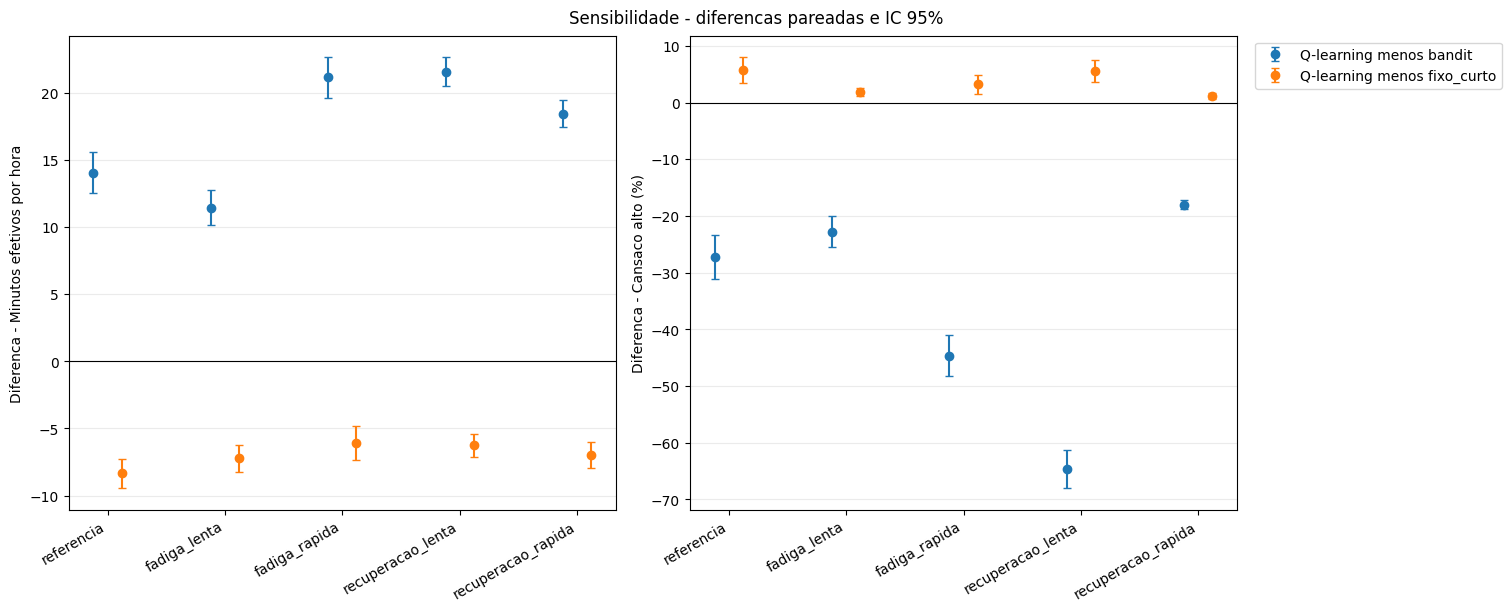
\includegraphics[width=\linewidth,height=.54\textheight,keepaspectratio]{figuras_pomodoro/sensibilidade.png}
\par\smallskip\raggedright
Na referência, o Q-learning ganha \textbf{14,04 min.\ efetivos/h} sobre o bandit (IC 95\% de 12,52 a 15,57) e perde \textbf{8,35 min.\ efetivos/h} para o curto fixo (diferença de $-9{,}45$ a $-7{,}24$ no IC).
\fonte{gráfico de diferenças pareadas salvo em \notebook}
\end{frame}

\begin{frame}{Com novo treino, como varia o cansaço alto?}
\centering\small
Diferença média em p.p. [IC de 95\%], por cenário de treino e avaliação.\par\medskip
\begin{tabular}{lrr}
\toprule Cenário & Q-learning menos bandit & Q-learning menos curto\\ \midrule
Referência & $-27{,}28$ [$-31{,}16$ a $-23{,}40$] & $+5{,}73$ [3,45 a 8,00]\\
Fadiga lenta & $-22{,}77$ [$-25{,}47$ a $-20{,}08$] & $+1{,}84$ [1,14 a 2,54]\\
Fadiga rápida & $-44{,}63$ [$-48{,}21$ a $-41{,}05$] & $+3{,}27$ [1,59 a 4,95]\\
Recuperação lenta & $-64{,}69$ [$-68{,}02$ a $-61{,}36$] & $+5{,}58$ [3,68 a 7,48]\\
Recuperação rápida & $-17{,}99$ [$-18{,}76$ a $-17{,}22$] & $+1{,}11$ [0,61 a 1,61]\\
\bottomrule
\end{tabular}
\begin{block}{Recuperação lenta}
A maior redução frente ao bandit ocorre quando a pausa alivia menos fadiga por minuto. Mesmo nesse cenário, o curto fixo registra menos cansaço alto que o Q-learning.
\end{block}
\fonte{diferenças por semente em \texttt{execucoes.csv}, com o IC calculado como em \notebook}
\end{frame}

\begin{frame}{Sem novo treino, a ordem das três políticas se mantém}
\centering
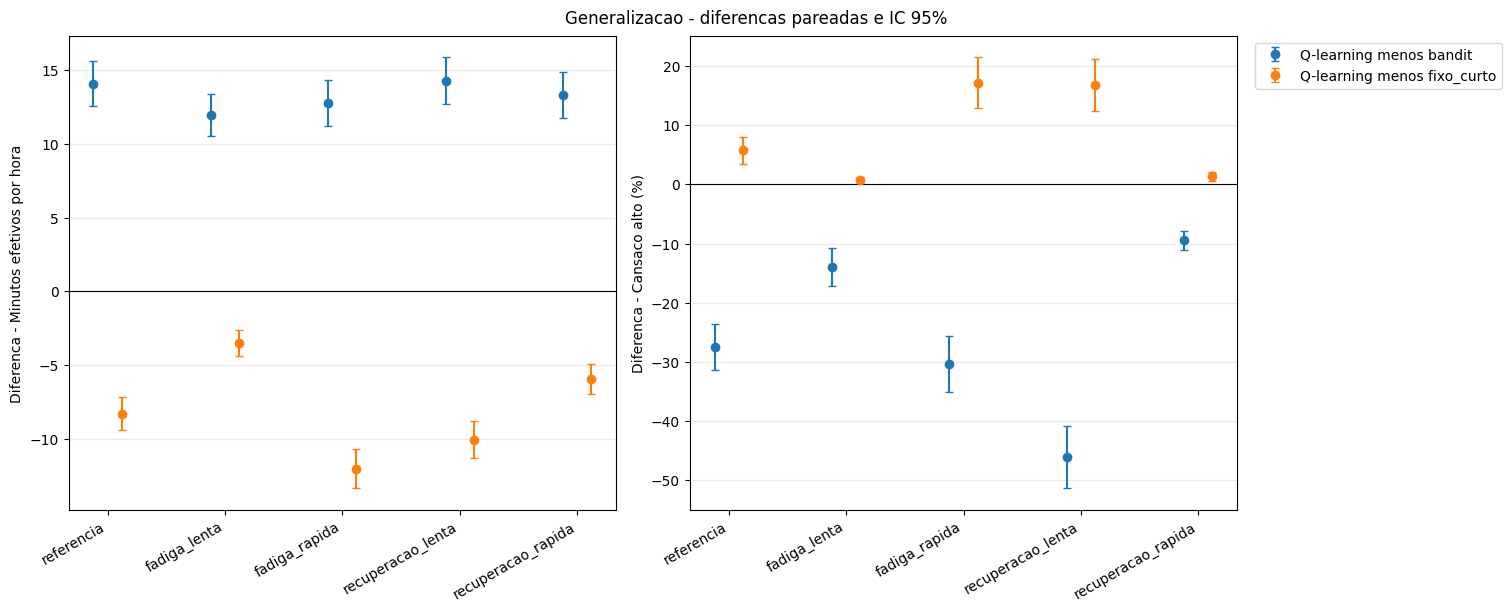
\includegraphics[width=\linewidth,height=.54\textheight,keepaspectratio]{figuras_pomodoro/generalizacao.png}
\par\smallskip\raggedright
As tabelas aprendidas na referência preservam a vantagem do Q-learning sobre o bandit nos cinco ambientes. O curto fixo ainda tem maior rendimento e menor frequência de cansaço alto que ambos.
\fonte{gráfico de diferenças pareadas da generalização salvo em \notebook}
\end{frame}

\begin{frame}{Onde a política treinada na referência fica mais atrás?}
\small
Na avaliação com \textbf{fadiga rápida}, as diferenças pareadas quantificam a vantagem sobre o bandit e a perda frente ao curto.\par\medskip
\centering
\begin{tabular}{lcc}
\toprule Diferença & Minutos efetivos/h [IC 95\%] & Cansaço em p.p. [IC 95\%]\\ \midrule
Q-learning menos bandit & $+12{,}75$ [11,20 a 14,31] & $-30{,}34$ [$-35{,}04$ a $-25{,}63$]\\
Q-learning menos curto & $-12{,}06$ [$-13{,}37$ a $-10{,}74$] & $+17{,}18$ [12,89 a 21,47]\\
\bottomrule
\end{tabular}
\begin{block}{Comparação entre protocolos}
Com novo treino nesse cenário, o excesso de cansaço frente ao curto foi de 3,27 p.p. As duas avaliações usam fluxos aleatórios distintos. O notebook não estima um IC direto para o efeito de treinar novamente.
\end{block}
\fonte{saídas pareadas de \notebook}
\end{frame}

\section{Discussão e conclusões}
\begin{frame}{Por que a recompensa e a avaliação podem divergir?}
\begin{block}{Uma sessão pode durar três vezes mais que outra}
O agente aprende com recompensas por bloco ao longo de oito decisões. Já o rendimento divide os minutos efetivos por todo o tempo de relógio. Um bloco pode somar mais pontos e, ainda assim, render menos por hora.
\end{block}
\begin{itemize}
\item Esse desalinhamento oferece uma hipótese para o desempenho do curto fixo. O experimento não mediu quanto da diferença ele explica.
\item A vantagem sobre o bandit é compatível com um benefício de considerar ciclos futuros. Sua magnitude também pode depender de exploração, convergência e hiperparâmetros.
\end{itemize}
\end{frame}

\begin{frame}{O que os resultados sustentam?}
\begin{alertblock}{Conclusão no simulador}
Nos cinco cenários e nos dois protocolos, o Q-learning rendeu mais e registrou menos cansaço alto que o bandit. O ciclo curto fixo superou o Q-learning nas mesmas duas métricas.
\end{alertblock}
\begin{itemize}
\item \textbf{Alcance.} Fadiga, eficiência e autorrelato seguem hipóteses do simulador. Os resultados não estimam aprendizagem ou cansaço em estudantes reais.
\item \textbf{Próximo teste.} Fixar a duração total da sessão e comparar recompensas alinhadas ao rendimento por hora.
\item \textbf{Robustez.} Combinar mudanças de fadiga e recuperação, variar o ruído do relato e examinar os ciclos escolhidos em cada estado.
\end{itemize}
\end{frame}
\end{document}
